\graphicspath{{./img}} % path to graphics

\section*{\LARGE Введение}
\addcontentsline{toc}{section}{Введение}
Компьютер работает в мультипрограммном режиме
обработки пакетов, т.е. одновременно начинает обработку
нескольких (вплоть до установленного максимума k = 4)
заданий, но не может начать обработку новых заданий,
пока не будет выполнен этот пакет. В пакете каждое
задание имеет собственное время выполнения, которое
покидает центральный процессор (ЦП) по его истечении. В
системе существует три класса приоритетов: высший
приоритет имеют задания типа 3, средний --- задания типа
2, низший --- задания типа 1. Когда ЦП завершает
выполнение последнего задания в пакете, он сначала
обращается к заданиям из очереди класса 3 и берет на
выполнение как можно больше заданий, вплоть до
указанного максимума k. Если в очереди класса 3 было
меньше k заданий, ЦП принимает как можно больше
заданий из очереди класса 2, чтобы сумма заданий класса
1 и класса 2 составила максимальный размер пакета k. Если
в пакете еще остается место, ЦП переходит к очереди класса
1. Процессор не может начать обработку любых
поступающих заданий, пока не завершит выполнение всех
заданий в текущем пакете.\par
Установленное время обслуживания задания класса \texttt{i}
равномерно распределено между константами \(a_i\) и \(b_i\). Для
каждого класса заданий действует отдельный процесс
поступления, т.е. интервалы времени между поступлениями
двух последовательных заданий класса i экспоненциально
распределены со средним значением \(r_i\).\par
Для моделирования логики модели будем использовать
компоненты \textit{Библиотеки моделирования процессов}.

\clearpage

\section*{\LARGE Выполнение практической работы}
\addcontentsline{toc}{section}{Выполнение практической работы}
Создадим новую модель с именем \texttt{Processor} и далее
--- свой тип заявки. Для этого перетащим в Main
элемент Тип заявки и выполним шаги по его
созданию.\par
Изменим имя агента на \textbf{Entity} (заявка). Откажемся от
предложения выбрать анимацию агента (позже создадим
свою). Добавим агенту один параметр priority
вещественного типа.\par
Агент \textbf{Entity} появился в структуре проекта как класс
модели. Щелкнем по нему. Раскроется закладка окна
графического редактора заявки. Добавим в него элемент
oval из палитры Презентация и настроим его свойства.\par
Создадим источник заявок первого типа (с
наименьшим приоритетом). Для этого поместим в модель
элемент \textbf{source} (источник). Переименуем в source1.
Настроим его свойства. В качестве новой заявки будет
фигурировать агент \texttt{Entity}. При подходе к выходу из
источника заявке будет назначаться приоритет, при этом
кружок-презентация заявки будет светло-зеленого цвета.\par
Аналогично создадим источники заявок с
приоритетом 2 и 3. Назовем их, соответственно, \textbf{source2} и
\textbf{source3}. В поле свойств Время между прибытиями для
источника \textbf{source2} запишем \texttt{exponential(1.6)}, а для
источника \textbf{source3}: \texttt{exponential(.2)}. Внесем соответствующие
изменения в код в поле Действия --- При подходе к выходу.
Из \textbf{source2} будут выходить кружки синего цвета, а из
\textbf{source3} --- красного.\par
Внесем в модель три параметра целого типа.
Назовем их \textbf{count\_1}, \textbf{count\_2}, \textbf{count\_3}.
В них будут сохраняться количество заявок соответствующего типа в
пакете. Для контроля общего числа заявок в пакете (их
должно быть ровно 4) понадобится еще один параметр –
\textbf{pack}.\par
Раскроем список элементов Разметка
пространства библиотеки процессов. Перетащим в модель
два элемента Прямоугольный узел.\par
Добавим в модель элементы \textbf{queue} (очередь), \textbf{hold}
(захват), \textbf{delay} (задержка), \textbf{sink} (сток). Далее
последовательно соединим их. Ко входу очереди подключим
источники заданий.\par
Настроим свойства очереди. В качестве места
заявок укажем элемент node.\par
Настроим работу процессора.\par
Полное время обработки пакета заданий будет
рассчитываться, исходя из количества попавших в него
заявок с соответствующим приоритетом. По мере выхода
заданий из блока \textbf{delay} счетчик соответствующей заявки,
попавшей на обработку, будет уменьшаться, пока не станет
равным нулю. После обработки всего пакета параметр \textbf{pack}
станет равен нулю и элемент \textbf{hold} будет разблокирован.
Затем заявки снова начнут поступать в процессор из
очереди до тех пор, пока не будет сформирован новый
пакет из четырех заданий. Для реализации пропишем
следующий код в свойстве При выходе блока \textbf{Delay}.\par
Полное время обработки пакета заданий будет
рассчитываться, исходя из количества попавших в него
заявок с соответствующим приоритетом. По мере выхода
заданий из блока \textbf{delay} счетчик соответствующей заявки,
попавшей на обработку, будет уменьшаться, пока не станет
равным нулю. После обработки всего пакета параметр \textbf{pack}
станет равен нулю и элемент \textbf{hold} будет разблокирован.
Затем заявки снова начнут поступать в процессор из
очереди до тех пор, пока не будет сформирован новый
пакет из четырех заданий. Для реализации пропишем
следующий код в свойстве При выходе блока \textbf{Delay}.\par
Для анализа динамических свойств модели
организуем сбор данных о работе очереди и процессора.\par
Запустим модель и проанализируем работу системы
(рис. \ref{fig:model:res}).

\begin{image}
	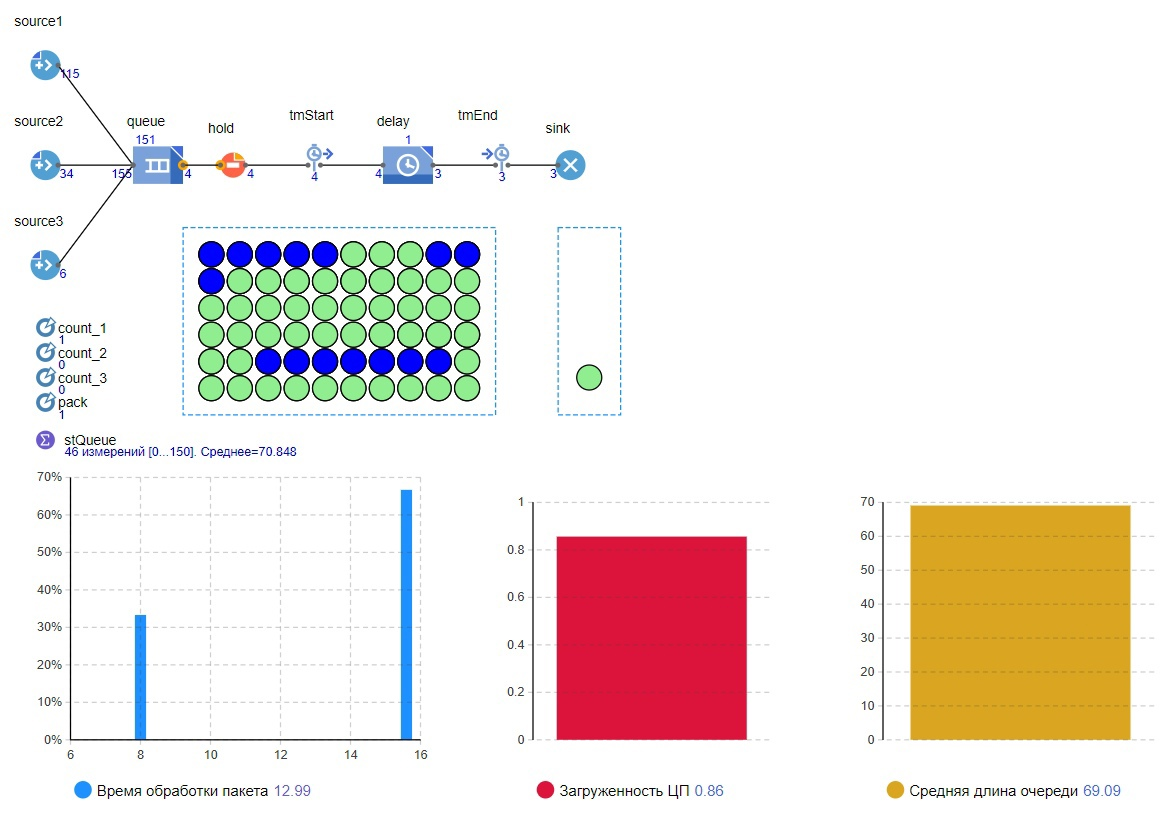
\includegraphics[width=0.9\textwidth]{model-result}
	\caption{Использование базы данных}
	\label{fig:model:res}
\end{image}

\clearpage

\section*{\LARGE Вывод}
\addcontentsline{toc}{section}{Вывод}
В данной практической работе была создана простая модель процессора.\par
При создании модели использовалась
\textbf{система массового обслуживания (СМО)}.
Другими примерами СМО могут служить:
орорганизация медицинских услуг пациентам в поликлинике;
банковское обслуживание клиентов; работа АЗС.
